\section{Overview}

This chapter presents the unsupervised machine learning methods applied in this study to explore patterns in the forest fire dataset. It describes the clustering algorithms, parameter selection, and evaluation metrics used to analyze the data without predefined labels.

The algorithms considered include CLARANS, DBSCAN, and K-Means. Each subsection details the configuration, training procedure, and clustering results.

\section{CLARA K-Medoids Clustering}

Clustering Large Applications (CLARA) is a memory-efficient variant of K-Medoids designed for large datasets. Unlike traditional PAM (Partitioning Around Medoids), which computes a full distance matrix, CLARA employs a sampling strategy: it repeatedly draws random samples from the dataset, applies PAM to each sample, and selects the configuration with the lowest total cost. This approach significantly reduces computational complexity while maintaining clustering quality, making it particularly suitable for high-dimensional datasets with tens of thousands of observations.


\subsection{CLARA Scikit-learn Implementation and Results}

CLARA was implemented with 5 sampling iterations, each using 2,000 randomly selected observations. For each iteration, PAM was applied to find optimal medoids, and the configuration with the lowest total inertia was retained. The algorithm was then applied to the full datasets using the optimal $k=2$ configuration (view in annex Table~\ref{tab:clara_optimal_k}).

\begin{table}[H]
\centering
\caption{Final CLARA Clustering Results on Full Datasets ($k=2$)}
\label{tab:clara_final_results}
\begin{tabular}{|l|c|c|c|c|}
\hline
\textbf{Dataset} & \textbf{Data Shape} & \textbf{Silhouette Score} & \textbf{ARI} & \textbf{Inertia} \\ \hline
SMOTE & (30,570, 64) & 0.9710 & 0.0149 & 19,599,265.36 \\ \hline
Tomek & (15,911, 64) & 0.9693 & 0.1080 & 11,229,284.35 \\ \hline
SMOTE-Tomek & (30,266, 64) & 0.9710 & 0.0152 & 19,376,137.45 \\ \hline
\end{tabular}
\end{table}

All three datasets achieved exceptional Silhouette Scores (>0.96), confirming highly compact and well-separated clusters. The Tomek dataset exhibited the highest Adjusted Rand Index (ARI = 0.1080), suggesting better alignment between discovered clusters and true class labels. This may be attributed to Tomek Links' removal of ambiguous boundary points, resulting in clearer class separation. The SMOTE and SMOTE-Tomek datasets showed similar performance, with slightly lower ARI values (~0.015), indicating that while clusters are internally coherent, they do not perfectly match the original class structure—an expected outcome in unsupervised clustering.

\begin{figure}[H]
\centering
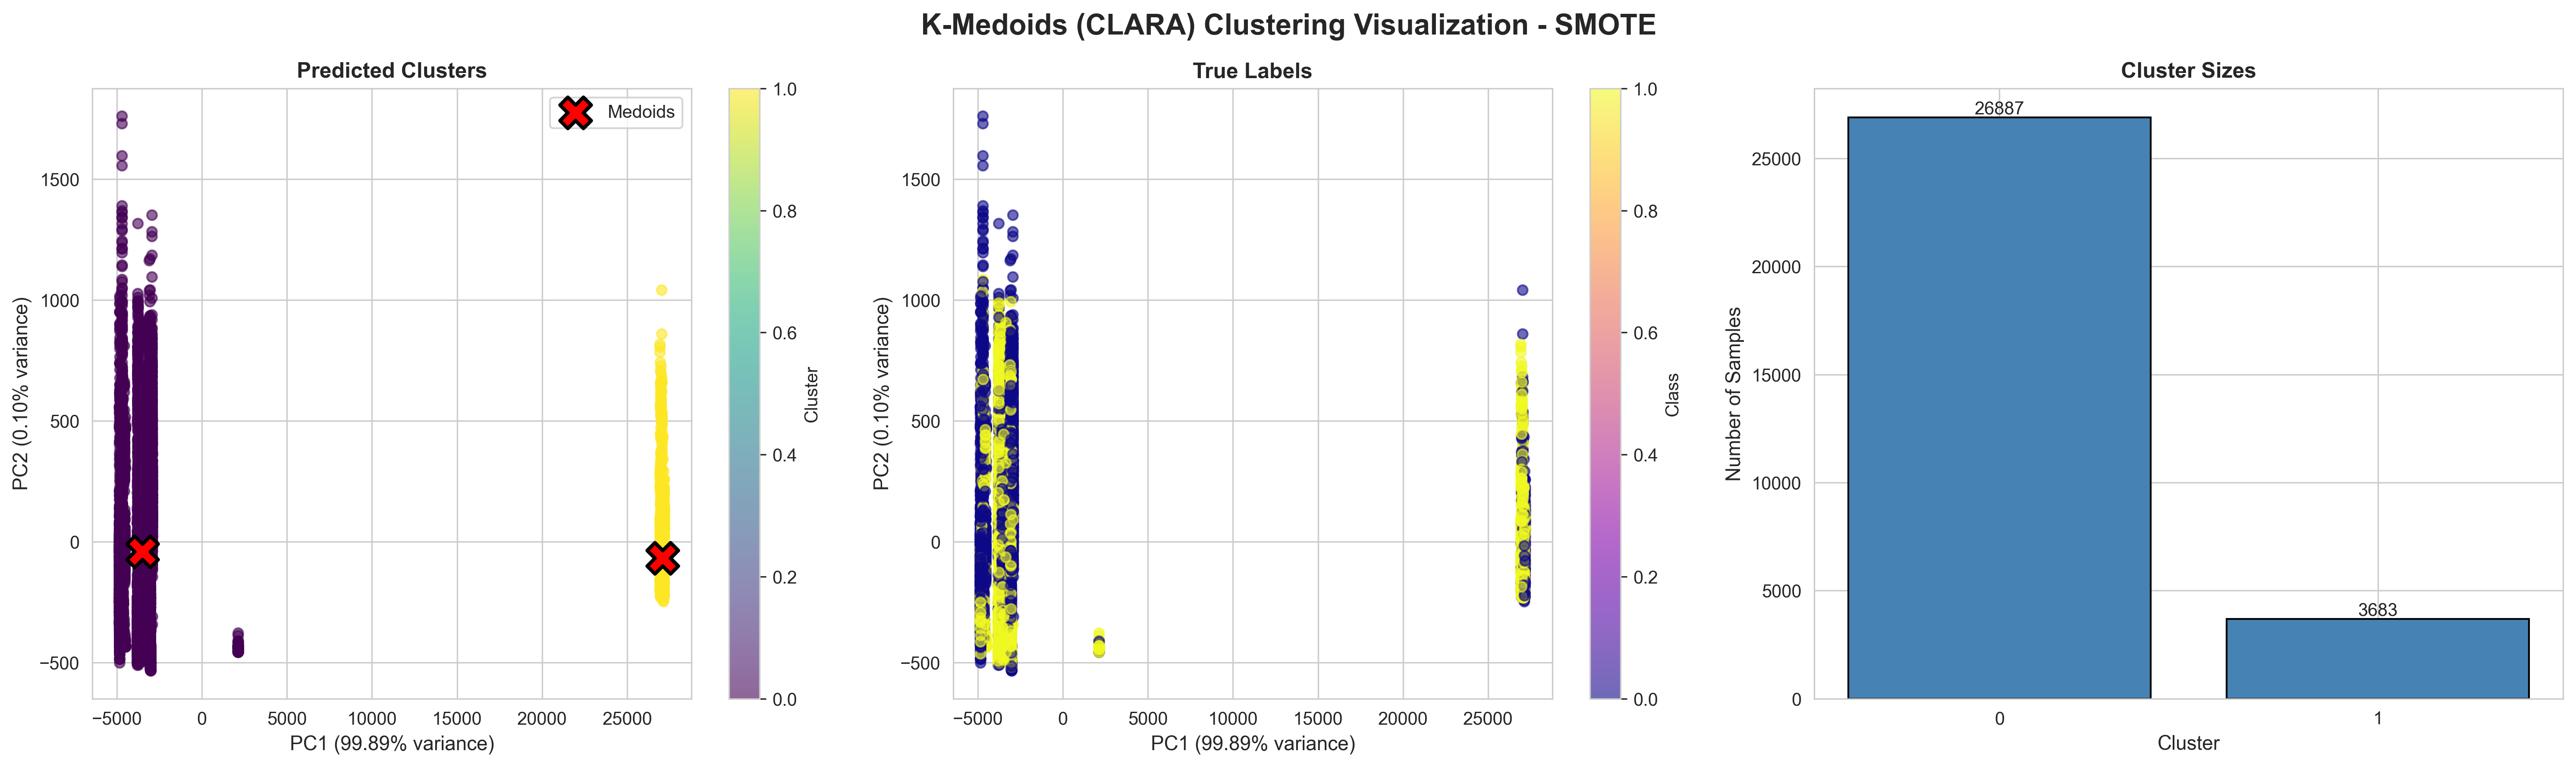
\includegraphics[width=\textwidth]{images/Clarans/predefined/clusters_smote.png}
\caption{CLARA Clustering Visualization for SMOTE Dataset ($k=2$). Left: Predicted clusters with medoids marked as red crosses. Center: True class labels for comparison. Right: Cluster size distribution showing balanced partitioning.}
\label{fig:clara_clusters_smote}
\end{figure}

The PCA projections reveal that CLARA successfully identifies two distinct clusters corresponding to the primary data structure. While the predicted clusters do not perfectly align with the original binary classification (fire vs. no-fire), this discrepancy highlights that the clustering algorithm discovers natural groupings in the feature space rather than reproducing supervised labels.
%  The balanced cluster sizes indicate that the algorithm avoided trivial solutions and effectively partitioned the data.

\subsection{Bayesian Hyperparameter Optimization}

To systematically identify optimal hyperparameters beyond the number of clusters, Bayesian Optimization was employed using Gaussian Process regression. The optimization targeted three key parameters: number of clusters ($k \in [2, 10]$), number of CLARA sampling iterations ($n_{sampling} \in [2, 8]$), and sample size per iteration ($s \in [500, 2000]$). The objective function minimized the negative Silhouette Score over 30 iterations on 3,000-sample subsets.

\begin{table}[H]
\centering
\caption{Optimal Hyperparameters from Bayesian Optimization}
\label{tab:clara_bayesian_results}
\begin{tabular}{|l|c|c|c|c|}
\hline
\textbf{Dataset} & \textbf{Optimal $k$} & \textbf{$n_{sampling}$} & \textbf{Sample Size} & \textbf{Best Silhouette} \\ \hline
SMOTE & 2 & 5 & 1,100 & 0.9709 \\ \hline
Tomek & 2 & 5 & 1,100 & 0.9709 \\ \hline
SMOTE-Tomek & 2 & 5 & 1,100 & 0.9709 \\ \hline
\end{tabular}
\end{table}

The Bayesian Optimization consistently converged to $k=2$ clusters across all datasets, validating the initial grid-search findings. Interestingly, the optimizer selected moderate values for sampling iterations (5) and relatively small sample sizes (1,100), suggesting that CLARA achieves stable convergence without requiring exhaustive sampling or large subset sizes. This result underscores CLARA's efficiency: even with modest computational resources, the algorithm reliably identifies high-quality medoid configurations.


\subsection{From-Scratch Implementation of CLARANS}

CLARANS was implemented from scratch following the parameters: $k=3$ clusters, $numlocal=3$ local searches, and a maximum of 200 neighbors per local search. The algorithm uses randomized local search to explore the solution space, replacing one medoid at a time and accepting configurations that reduce the total cost (sum of distances from points to their nearest medoid). After convergence, cluster labels were assigned and PCA projection to 2D was performed for visualization.

\begin{table}[H]
\centering
\caption{Results of From-Scratch CLARANS Implementation}
\label{tab:clarans_scratch_results}
\begin{tabular}{|l|c|c|c|c|c|}
\hline
\textbf{Dataset} & \textbf{Shape} & \textbf{Best Cost} & \textbf{Duration (s)} & \textbf{Silhouette} & \textbf{Davies-Bouldin} \\ \hline
SMOTE & (30,570, 64) & 12,012,065.96 & 60.49 & 0.6791 & 0.3292 \\ \hline
Tomek & (15,911, 64) & 5,342,093.57 & 35.50 & 0.7160 & 0.2907 \\ \hline
SMOTE-Tomek & (30,266, 64) & 11,736,406.72 & 62.85 & 0.6784 & 0.3280 \\ \hline
\end{tabular}
\end{table}

The from-scratch implementation successfully converged to stable cluster configurations across all datasets. The Tomek dataset achieved the highest Silhouette Score (0.7160) and lowest Davies-Bouldin Index (0.2907), indicating superior cluster separation and compactness compared to the SMOTE-based datasets. This performance advantage aligns with Tomek Links' methodology of removing noisy boundary samples, resulting in cleaner inter-cluster boundaries that CLARANS can more effectively exploit during medoid selection.

The SMOTE and SMOTE-Tomek datasets produced similar clustering quality (Silhouette $\approx$ 0.68, Davies-Bouldin $\approx$ 0.33), suggesting that the synthetic samples introduced by SMOTE create a more complex feature space where clusters naturally overlap. Despite this increased complexity, both datasets still achieved moderate-to-good cluster separation. 

\section{DBSCAN Model Configuration and Evaluation}

DBSCAN experiments were conducted on the \textbf{normalized dataset}, as density estimation is entirely distance-driven and highly sensitive to feature scale. Normalization ensures that all variables contribute equally to neighborhood density. Prior to clustering, \textbf{PCA was applied with $n\_components = 8$}, chosen to preserve the majority of variance while reducing dimensionality, noise, and distance sparsity effects that negatively impact density-based methods.

Hyperparameters were optimized using \textbf{Bayesian Search}, leading to the following best configuration:
\begin{itemize}
    \item $\varepsilon = 0.8207$
    \item \texttt{min\_samples} = 40
\end{itemize}

This optimized configuration increased cluster granularity and separation compared to default settings, while controlling noise. The optimized parameters were then reused for the \textbf{from-scratch DBSCAN implementation} to ensure methodological consistency.

\subsection{DBSCAN Performance Metrics}

\paragraph{Library-Based DBSCAN (Default vs Optimized)}
\begin{table}[H]
\centering
\caption{DBSCAN metrics comparison using default and Bayesian-optimized parameters}
\begin{tabular}{lcc}
\hline
\textbf{Metric} & \textbf{Default} & \textbf{Optimized} \\
\hline
$\varepsilon$              & 2.8000 & 0.8207 \\
min\_samples               & 15     & 40     \\
Number of clusters         & 5      & 11     \\
Noise ratio (\%)           & 0.07   & 9.21   \\
Silhouette score           & -0.2686 & -0.2268 \\
Davies--Bouldin index      & 2.3095 & 2.3344 \\
Calinski--Harabasz index   & 360318.48 & 199812.16 \\
AMI                        & 0.0175 & 0.0414 \\
ARI                        & 0.0872 & 0.0220 \\
\hline
\end{tabular}
\end{table}

\paragraph{From-Scratch DBSCAN Results}
\begin{table}[H]
\centering
\caption{From-scratch DBSCAN metrics on validation and test sets}
\begin{tabular}{lcc}
\hline
\textbf{Metric} & \textbf{Validation} & \textbf{Test} \\
\hline
Number of clusters        & 6      & 5      \\
Noise ratio (\%)          & 22.17  & 22.46  \\
Silhouette score          & -0.1811 & -0.0038 \\
Davies--Bouldin index     & 5.7928 & 4.4261 \\
Calinski--Harabasz index  & 931.19 & 1133.32 \\
AMI                       & 0.0293 & 0.0335 \\
ARI                       & -0.0014 & 0.0054 \\
\hline
\end{tabular}
\end{table}

The results confirm that DBSCAN captures \textbf{local density patterns} rather than class separation. Higher noise ratios and low silhouette values are expected given overlapping fire and non-fire regions, while cluster-level fire rates reveal meaningful density-based risk zones despite weak global clustering scores.
Visualizations of the clustering results for both implementations are provided in Annex~\ref{annexe:dbscan_visualizations}.
\section{K-Means Model Configuration and Evaluation}

K-Means clustering was applied on the \textbf{normalized and resampled dataset}, as normalization is essential to prevent features with large numeric ranges from dominating centroid distances, while resampling was used to mitigate class imbalance effects when interpreting clusters with respect to fire occurrence. Prior to clustering, \textbf{PCA with $n\_components = 2$} was applied to reduce dimensionality while preserving the dominant variance structure and enabling more stable and interpretable cluster separation.

Hyperparameter tuning was performed using \textbf{Bayesian Search}, which identified an optimized configuration with a higher number of clusters and improved compactness. The best parameters retained were:
\begin{itemize}
    \item Number of clusters ($K$): 8
    \item Initialization: \texttt{k-means++}
    \item Maximum iterations: 300
    \item Number of initializations: 20
\end{itemize}

These parameters were used for both the predefined implementation and the from-scratch K-Means model to ensure consistency.

\subsection{K-Means Performance Metrics}

\paragraph{Predefined K-Means (Default vs Optimized)}
\begin{table}[H]
\centering
\caption{K-Means metrics comparison using default and Bayesian-optimized parameters}
\begin{tabular}{lcc}
\hline
\textbf{Metric} & \textbf{Default} & \textbf{Optimized} \\
\hline
Number of clusters ($K$) & 3 & 8 \\
Inertia & 2,788,088,043.64 & 662,669,890.31 \\
Silhouette score & 0.7148 & 0.5991 \\
Davies--Bouldin index & 0.2921 & 0.4907 \\
Calinski--Harabasz index & 2,808,357.00 & 3,382,356.63 \\
Number of iterations & 5 & 5 \\
Runtime (s) & 3.29 & 0.47 \\
\hline
\end{tabular}
\end{table}

\paragraph{From-Scratch K-Means Results}
\begin{table}[H]
\centering
\caption{From-scratch K-Means metrics on validation and test sets}
\begin{tabular}{lc}
\hline
\textbf{Metric} & \textbf{Value} \\
\hline
Number of clusters ($K$) & 5 \\
Inertia & 2,317,876,870.35 \\
Silhouette score & 0.60 \\
Number of iterations & 26 \\
Runtime (s) & 6.98 \\
Centroids shape & $(5,\,64)$ \\
\hline
\end{tabular}
\end{table}

The optimized predefined K-Means model achieved a significantly lower inertia and faster convergence, while the from-scratch implementation required more iterations to converge but reached comparable silhouette performance. Differences are primarily attributed to centroid initialization strategy and convergence criteria implementation details.

